% =====================================================================
\chapter{Entropía relativa e información mutua}
\label{tema:2}
% =====================================================================

Este tema introduce la entropía relativa o divergencia de Kullback--Leibler, que mide el coste de usar una distribución equivocada, y la información mutua, que mide cuánto informa una variable sobre otra. El resultado que lo articula todo es la desigualdad de Gibbs, que se deduce de la desigualdad de Jensen. Se sigue~\cite[§2.3--2.6 y §2.8]{ct}; la interpretación de las dos direcciones de la divergencia en aprendizaje automático procede del tema «Comparing probability distributions and machine learning» de~\cite{camit}, y la de la información mutua, de~\cite[cap.~8]{mackay}.

\section{La desigualdad de Jensen}

\begin{definicion}[Función convexa]\label{def:convexa}
Sea $I\subseteq\R$ un intervalo. Una función $f\colon I\to\R$ es \emph{convexa} si
\[
f\bigl(\lambda a+(1-\lambda)b\bigr)\le\lambda f(a)+(1-\lambda)f(b)\qquad\text{para todo }a,b\in I,\ \lambda\in[0,1],
\]
y \emph{estrictamente convexa} si la desigualdad es estricta cuando $a\ne b$ y $\lambda\in(0,1)$. La función $f$ es (estrictamente) \emph{cóncava} si $-f$ es (estrictamente) convexa.
\end{definicion}

Si $f$ es dos veces derivable con $f''\ge 0$ ($f''>0$) en $I$, entonces es convexa (estrictamente convexa)~\cite[§2.6]{ct}; el módulo~4 estudia este criterio. Así, $\ln$ y $\log$ son estrictamente cóncavas en $(0,\infty)$, porque $(\ln t)''=-1/t^{2}<0$, y $t\mapsto t\log t$ es estrictamente convexa en $(0,\infty)$.

\begin{teorema}[Desigualdad de Jensen]\label{teo:jensen}
Sea $f$ convexa en un intervalo $I$ y sea $X$ una variable aleatoria con valores en $I$ que toma un número finito de valores. Entonces
\[
\E[f(X)]\ge f\bigl(\E[X]\bigr).
\]
Si $f$ es estrictamente convexa, la igualdad se da si y solo si $X$ es constante con probabilidad~1. Para $f$ cóncava la desigualdad se invierte.
\end{teorema}

\begin{proof}
Por inducción sobre el número $m$ de valores con probabilidad positiva, $x_1,\dots,x_m$ con probabilidades $p_1,\dots,p_m$. Si $m=1$, ambos miembros valen $f(x_1)$. Si $m=2$, el enunciado es la definición de convexidad con $\lambda=p_1$. Supóngase cierto para $m-1$ valores y sea $p'_i=p_i/(1-p_m)$ para $i\le m-1$, que es una distribución. Entonces
\begin{align*}
\sum_{i=1}^{m}p_if(x_i)&=p_mf(x_m)+(1-p_m)\sum_{i=1}^{m-1}p'_if(x_i)\\
&\ge p_mf(x_m)+(1-p_m)f\Bigl(\sum_{i=1}^{m-1}p'_ix_i\Bigr)
\ge f\Bigl(p_mx_m+(1-p_m)\sum_{i=1}^{m-1}p'_ix_i\Bigr),
\end{align*}
por la hipótesis de inducción y por la convexidad, respectivamente; el último argumento es $\sum_i p_ix_i=\E[X]$. Si $f$ es estrictamente convexa y $m\ge 2$, la segunda desigualdad es estricta salvo que $x_m=\sum_{i<m}p'_ix_i$, y la primera es estricta salvo que los $x_i$ con $i<m$ coincidan; ambas igualdades juntas obligan a que todos los $x_i$ sean iguales, en contra de que sean $m\ge 2$ valores distintos.
\end{proof}

\section{Entropía relativa}

\begin{definicion}[Entropía relativa]\label{def:kl}
Sean $p$ y $q$ distribuciones sobre $\X$. La \emph{entropía relativa} o \emph{divergencia de Kullback--Leibler} de $p$ respecto de $q$ es
\[
\KL{p}{q}=\sum_{x\in\X}p(x)\log\frac{p(x)}{q(x)}=\E_{X\sim p}\Bigl[\log\frac{p(X)}{q(X)}\Bigr],
\]
con los convenios $0\log\frac{0}{q}=0$ y $p\log\frac{p}{0}=+\infty$ si $p>0$.
\end{definicion}

En particular, $\KL{p}{q}=+\infty$ en cuanto $q$ declara imposible un resultado que, según $p$, puede ocurrir. Es la versión informacional de la pérdida infinita del módulo~1 cuando un modelo asigna probabilidad~0 a un token del texto.

\begin{teorema}[Desigualdad de Gibbs o de la información]\label{teo:gibbs}
Para distribuciones $p$ y $q$ sobre $\X$, $\KL{p}{q}\ge 0$, con igualdad si y solo si $p=q$.
\end{teorema}

\begin{proof}
Si $\KL{p}{q}=+\infty$ no hay nada que probar. En otro caso, sea $S=\{x:p(x)>0\}$, sobre el que $q(x)>0$. Aplicando la desigualdad de Jensen a la función cóncava $\log$ y a la variable $q(X)/p(X)$ con $X\sim p$,
\[
-\KL{p}{q}=\sum_{x\in S}p(x)\log\frac{q(x)}{p(x)}\le\log\sum_{x\in S}p(x)\frac{q(x)}{p(x)}=\log\sum_{x\in S}q(x)\le\log 1=0.
\]
Como $\log$ es estrictamente cóncava, la primera desigualdad es una igualdad si y solo si $q(x)/p(x)$ es constante en $S$; la segunda lo es si y solo si $\sum_{x\in S}q(x)=1$. Si ambas se cumplen, la constante es~1 y $q=p$. El recíproco es inmediato~\cite[teorema~2.6.3]{ct}.
\end{proof}

\begin{ejemplo}[Asimetría]\label{ej:asimetria}
Sean $p=(0{,}5;\ 0{,}25;\ 0{,}25)$ y $q=(0{,}8;\ 0{,}1;\ 0{,}1)$. Entonces
\[
\KL{p}{q}=0{,}5\log\tfrac{0{,}5}{0{,}8}+2\cdot 0{,}25\log\tfrac{0{,}25}{0{,}1}=-0{,}3390+0{,}6610=0{,}322\text{ bits},
\]
mientras que $\KL{q}{p}=0{,}8\log 1{,}6+2\cdot 0{,}1\log 0{,}4=0{,}5425-0{,}2644=0{,}278$ bits.
\end{ejemplo}

\begin{observacion}
La entropía relativa no es simétrica y no cumple la desigualdad triangular; por eso se llama \emph{divergencia} y no distancia. Sí cumple la propiedad que importa para comparar un modelo con los datos: es no negativa y solo se anula cuando las dos distribuciones coinciden.
\end{observacion}

\section{Entropía cruzada}

\begin{definicion}[Entropía cruzada]\label{def:cruzada}
La \emph{entropía cruzada} de $q$ respecto de $p$ es $H(p,q)=-\sum_{x}p(x)\log q(x)=\E_{X\sim p}[-\log q(X)]$.
\end{definicion}

\begin{proposicion}[Descomposición de la entropía cruzada]\label{prop:descomposicion}
$H(p,q)=H(p)+\KL{p}{q}$. En consecuencia, $H(p,q)\ge H(p)$, con igualdad si y solo si $q=p$.
\end{proposicion}

\begin{proof}
En cada término con $p(x)>0$, $-\log q(x)=-\log p(x)+\log\bigl(p(x)/q(x)\bigr)$. Multiplicando por $p(x)$ y sumando se obtiene la identidad. La desigualdad se sigue del \cref{teo:gibbs}.
\end{proof}

En el \cref{ej:asimetria}, $H(p)=1{,}5$ bits y $H(p,q)=1{,}822$ bits, cuya diferencia es $\KL{p}{q}=0{,}322$ bits. El \cref{tema:3} dará a esta identidad un sentido operativo: $H(p,q)$ es la longitud media de un código diseñado para $q$ cuando los datos siguen $p$, y $\KL{p}{q}$ son los bits que se desperdician por usar el modelo equivocado.

\begin{observacion}[Conexión con los LLM]
Sea $p$ la distribución del texto real y $q_\theta$ el modelo. La pérdida de preentrenamiento es una estimación de
\[
\underbrace{H(p,q_\theta)}_{\text{pérdida}}=\underbrace{H(p)}_{\text{irreducible}}+\underbrace{\KL{p}{q_\theta}}_{\text{mejorable}}.
\]
Como $H(p)$ no depende de $\theta$, minimizar la entropía cruzada equivale a minimizar $\KL{p}{q_\theta}$, y la pérdida nunca baja de $H(p)$. Las leyes de escalado de Hoffmann \emph{et al.}~\cite{chinchilla} (módulo~16) incluyen un término constante $E$ que los autores interpretan como la entropía del texto natural.
\end{observacion}

\begin{observacion}[Las dos direcciones de la divergencia]\label{obs:direcciones}
Al ajustar una distribución $q$ a una distribución $p$ dada pueden minimizarse dos cantidades distintas. La divergencia \emph{hacia delante} $\KL{p}{q}$ penaliza con fuerza que $q(x)$ sea pequeña donde $p(x)$ no lo es: $q$ tiende a \emph{cubrir} todo el soporte de $p$. Es la que se minimiza al entrenar por máxima verosimilitud. La divergencia \emph{hacia atrás} $\KL{q}{p}$ penaliza que $q$ ponga masa donde $p$ es pequeña: $q$ tiende a \emph{concentrarse} en una de las modas de $p$. Es la que aparece en la inferencia variacional y en la penalización del ajuste por preferencias del \cref{tema:5}~\cite{camit}.
\end{observacion}

\section{Información mutua}

\begin{definicion}[Información mutua]\label{def:mutua}
La \emph{información mutua} entre $X$ e $Y$ es la entropía relativa entre la distribución conjunta y el producto de las marginales:
\[
I(X;Y)=\KL{p(x,y)}{p(x)\,p(y)}=\sum_{x,y}p(x,y)\log\frac{p(x,y)}{p(x)\,p(y)}.
\]
\end{definicion}

\begin{proposicion}\label{prop:mutua-identidades}
\[
I(X;Y)=H(X)+H(Y)-H(X,Y)=H(Y)-H(Y\mid X)=H(X)-H(X\mid Y).
\]
En particular, $I(X;Y)=I(Y;X)$ e $I(X;X)=H(X)$.
\end{proposicion}

La demostración de la primera igualdad se propone en el \cref{eje:2-mutua}; las otras dos se siguen de ella y de la regla de la cadena (\cref{teo:cadena-entropia}). Para $Y=X$ se tiene $H(X\mid X)=0$.

\begin{teorema}\label{teo:mutua-positiva}
$I(X;Y)\ge 0$, con igualdad si y solo si $X$ e $Y$ son independientes. En consecuencia, $H(Y\mid X)\le H(Y)$: condicionar no aumenta, en media, la entropía.
\end{teorema}

\begin{proof}
Por la \cref{def:mutua} y el \cref{teo:gibbs}, $I(X;Y)\ge 0$, con igualdad si y solo si $p(x,y)=p(x)p(y)$ para todo par, que es la definición de independencia. La segunda afirmación se sigue de $I(X;Y)=H(Y)-H(Y\mid X)$.
\end{proof}

\begin{observacion}
La desigualdad $H(Y\mid X)\le H(Y)$ vale en media, no para cada valor: puede ocurrir $H(Y\mid X=x)>H(Y)$ para algún $x$ concreto. Una observación sorprendente puede aumentar la incertidumbre, aunque observar $X$ la reduce en promedio~\cite[§2.6]{ct}.
\end{observacion}

\begin{figure}[h]
\centering
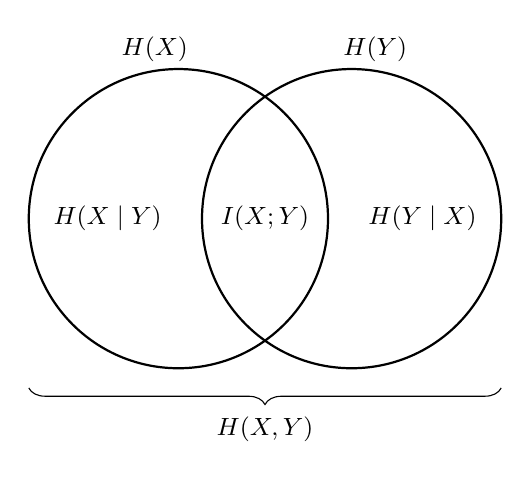
\begin{tikzpicture}[font=\small]
  \draw[thick] (0,0) circle (1.9cm);
  \draw[thick] (2.2,0) circle (1.9cm);
  \node at (-0.9,0) {$H(X\mid Y)$};
  \node at (1.1,0) {$I(X;Y)$};
  \node at (3.1,0) {$H(Y\mid X)$};
  \node at (-0.3,2.15) {$H(X)$};
  \node at (2.5,2.15) {$H(Y)$};
  \draw[decorate,decoration={brace,mirror,amplitude=6pt}] (-1.9,-2.15) -- (4.1,-2.15) node[midway,below=7pt] {$H(X,Y)$};
\end{tikzpicture}
\caption{Relaciones entre entropías e información mutua. Cada círculo representa la entropía de una variable; la intersección es la información compartida y la unión, la entropía conjunta.}
\label{fig:venn}
\end{figure}

\begin{ejemplo}\label{ej:mutua-bits}
Para los dos bits del \cref{ej:dos-bits}, $I(X;Y)=H(X)+H(Y)-H(X,Y)=2-1{,}722=0{,}278$ bits y $H(X\mid Y)=1-0{,}278=0{,}722$ bits. Conocer uno de los bits elimina algo más de una cuarta parte de la incertidumbre sobre el otro.
\end{ejemplo}

\begin{observacion}[Conexión con los LLM]
La información mutua entre el contexto $X_{1:t-1}$ y el token siguiente $X_t$ es la reducción de la incertidumbre sobre $X_t$ que puede lograr un modelo que vea ese contexto: $H(X_t\mid X_{1:t-1})=H(X_t)-I(X_t;X_{1:t-1})$. Un modelo de bigramas aprovecha solo $I(X_t;X_{t-1})$; un Transformer con miles de tokens de contexto puede aprovechar mucha más.
\end{observacion}

\section{La desigualdad del procesamiento de datos}

\begin{definicion}[Información mutua condicionada]
Para variables $X$, $Y$ y $Z$, la \emph{información mutua entre $X$ e $Y$ condicionada a $Z$} es $I(X;Y\mid Z)=H(X\mid Z)-H(X\mid Y,Z)$, donde $H(X\mid Y,Z)$ es la entropía de $X$ condicionada al par $(Y,Z)$.
\end{definicion}

Se cumple $I(X;Y\mid Z)=\sum_z p(z)\,I(X;Y\mid Z=z)\ge 0$, porque cada sumando es la información mutua de la distribución condicionada a $Z=z$ y es no negativo por el \cref{teo:mutua-positiva}. Además, aplicando la regla de la cadena a $H(X)-H(X\mid Y,Z)=\bigl[H(X)-H(X\mid Z)\bigr]+\bigl[H(X\mid Z)-H(X\mid Y,Z)\bigr]$ se obtiene la \emph{regla de la cadena para la información mutua}~\cite[§2.5]{ct}:
\[
I(X;Y,Z)=I(X;Z)+I(X;Y\mid Z).
\]

\begin{definicion}[Cadena de Markov]
Las variables $X$, $Y$ y $Z$ forman una \emph{cadena de Markov} $X\to Y\to Z$ si $p(z\mid x,y)=p(z\mid y)$ para todo $x,y,z$; es decir, si $Z$ depende de $X$ solo a través de $Y$. Esto equivale a que $X$ y $Z$ sean condicionalmente independientes dado $Y$, y en ese caso $I(X;Z\mid Y)=0$.
\end{definicion}

\begin{teorema}[Desigualdad del procesamiento de datos]\label{teo:procesamiento}
Si $X\to Y\to Z$, entonces $I(X;Z)\le I(X;Y)$.
\end{teorema}

\begin{proof}
Por la regla de la cadena aplicada en los dos órdenes,
\[
I(X;Y,Z)=I(X;Z)+I(X;Y\mid Z)=I(X;Y)+I(X;Z\mid Y).
\]
Por la hipótesis de Markov, $I(X;Z\mid Y)=0$, de modo que $I(X;Y)=I(X;Z)+I(X;Y\mid Z)\ge I(X;Z)$~\cite[§2.8]{ct}.
\end{proof}

\begin{corolario}\label{cor:procesamiento-funcion}
Para toda función $g$, $I(X;g(Y))\le I(X;Y)$.
\end{corolario}

\begin{proof}
$X\to Y\to g(Y)$ es una cadena de Markov, porque $g(Y)$ queda determinada por $Y$.
\end{proof}

\begin{observacion}
Ningún procesamiento de un dato, por elaborado que sea, aumenta la información que contiene sobre otra variable. Las representaciones internas de una red neuronal son funciones de su entrada; por el \cref{cor:procesamiento-funcion}, no contienen más información sobre la respuesta correcta que la propia entrada. Lo que el entrenamiento consigue es hacer esa información \emph{accesible} para una capa de salida sencilla, no crearla.
\end{observacion}

\begin{lecturas}
\item Cover y Thomas~\cite{ct}, §2.3 «Relative Entropy and Mutual Information», §2.4 «Relationship Between Entropy and Mutual Information», §2.6 «Jensen's Inequality and Its Consequences» y §2.8 «Data-Processing Inequality».
\item MacKay~\cite{mackay}, cap.~2 (desigualdad de Gibbs y de Jensen) y cap.~8 «Correlated Random Variables».
\item Universidad de Cambridge, \emph{Information Theory}~\cite{camit}, temas «Entropy of discrete variables» y «Comparing probability distributions and machine learning».
\item MIT 6.441~\cite{mit6441}, notas de clase sobre entropía, divergencia e información mutua.
\end{lecturas}

\section*{Ejercicios del tema 2}
\addcontentsline{toc}{section}{Ejercicios del tema 2}

\begin{ejercicio}{1}{eje:2-vf}
Justifique si son verdaderas o falsas: (a) $\KL{p}{q}=\KL{q}{p}$ para todo par de distribuciones; (b) $H(p,q)\ge H(p)$; (c) la entropía de una distribución sobre 4 símbolos puede valer 3 bits; (d) si $I(X;Y)=0$, entonces $X$ e $Y$ son independientes.
\end{ejercicio}

\begin{ejercicio}{1}{eje:2-direcciones}
(a) Explique por qué la entropía relativa se llama divergencia y no distancia. (b) Sea $p$ una distribución con dos modas separadas y sea $q$ una distribución de una familia que solo admite una moda. Describa cómo será, cualitativamente, la $q$ que minimiza $\KL{p}{q}$ y la que minimiza $\KL{q}{p}$, y diga cuál de las dos se minimiza al entrenar un modelo de lenguaje por máxima verosimilitud.
\fuente{adaptado de Universidad de Cambridge, \emph{Information Theory}~\cite{camit}, \emph{Examples Sheet}, \emph{Supervision}~3, ejercicios~10 y~11.}
\end{ejercicio}

\begin{ejercicio}{2}{eje:2-kl-moneda}
Sean $p=(1/2,1/2)$ los datos y $q=(0{,}9;\ 0{,}1)$ el modelo. Calcule $H(p,q)$, $\KL{p}{q}$ y $\KL{q}{p}$ en bits.
\end{ejercicio}

\begin{ejercicio}{2}{eje:2-conjunta}
La distribución conjunta de dos bits es $p(0,0)=0{,}3$, $p(0,1)=0{,}2$, $p(1,0)=0{,}1$ y $p(1,1)=0{,}4$. Calcule $H(X)$, $H(Y)$, $H(X,Y)$, $I(X;Y)$ y $H(Y\mid X)$.
\end{ejercicio}

\begin{ejercicio}{2}{eje:2-galletas}
Un tarro contiene 6 galletas: 3 de cacahuete (C), 2 de chocolate (H) y 1 de avena (A). Bob se las come de una en una, eligiendo cada vez al azar entre las que quedan. Sean $X$ e $Y$ los sabores de la primera y de la segunda galleta. (a) Calcule $H(X)$, $H(Y)$, $H(X,Y)$, $H(Y\mid X)$, $H(X\mid Y)$ e $I(X;Y)$. (b) Calcule $\KL{P_{Y\mid X=\mathrm{H}}}{P_{Y\mid X=\mathrm{A}}}$ y $\KL{P_{Y\mid X=\mathrm{A}}}{P_{Y\mid X=\mathrm{H}}}$. (c) ¿Cuántos bits de información contiene el orden completo de los sabores?
\fuente{adaptado de MIT 6.441~\cite{mit6441}, \emph{Problem Set}~1, problema~1 (se omite el apartado en que $Y$ es la última galleta).}
\end{ejercicio}

\begin{ejercicio}{3}{eje:2-gibbs-ln}
(a) Demuestre el \cref{teo:gibbs} sin usar la desigualdad de Jensen, mediante la desigualdad $\ln t\le t-1$ para $t>0$, con igualdad solo en $t=1$. (b) Aplique el resultado a $\KL{p}{u}$, con $u$ la distribución uniforme sobre $K$ símbolos, para demostrar que $H(p)\le\log K$, con igualdad si y solo si $p=u$.
\end{ejercicio}

\begin{ejercicio}{3}{eje:2-mutua}
Demuestre que $I(X;Y)=H(X)+H(Y)-H(X,Y)$ a partir de la \cref{def:mutua} y deduzca que $H(Y\mid X)\le H(Y)$.
\end{ejercicio}
